\documentclass[
  a4paper,
  oneside,
  BCOR = 10mm,
  DIV = 12,
  12pt,
  headings = normal,
]{scrartcl}

%%% Length calculations
\usepackage{calc}
%%%

%%% Support for color
\usepackage{xcolor}
\definecolor{lightblue}{HTML}{03A9F4}
\definecolor{red}{HTML}{F44336}
%%%

%%% Including graphics
\usepackage{graphicx}
%%%

%%% Font selection
\usepackage{fontspec}

\setromanfont{STIX Two Text}[
  SmallCapsFeatures = {LetterSpace = 8},
]

\setsansfont{IBM Plex Sans}[
  Scale = MatchUppercase,
]

\setmonofont{IBM Plex Mono}[
  Scale = MatchUppercase,
]
%%%

%%% Math typesetting
\usepackage{amsmath}

\usepackage{unicode-math}
\setmathfont{STIX Two Math}

\usepackage{IEEEtrantools}
%%%

%%% List settings
\usepackage{enumitem}
\setlist[enumerate]{
  label*      = {\arabic*.},
  left        = \parindent,
  topsep      = 0\baselineskip,
  parsep      = 0\baselineskip,
  noitemsep, % override itemsep
}
% List settings for levels 2–4
\setlist[enumerate, 2, 3, 4]{
  label*      = {\arabic*.},
  left        = 0em,
  topsep      = 0\baselineskip,
  parsep      = 0\baselineskip,
  noitemsep, % override itemsep
}

\setlist[itemize]{
  label*      = {—},
  left        = \parindent,
  topsep      = 0\baselineskip,
  parsep      = 0\baselineskip,
  itemsep     = 1\baselineskip,
  noitemsep, % override itemsep
}

\setlist[description]{
  font        = {\rmfamily\upshape\bfseries},
  topsep      = 1\baselineskip,
  parsep      = 0\baselineskip,
  itemsep     = 0\baselineskip,
}

%%%

%%% Structural elements typesetting
\setkomafont{pagenumber}{\rmfamily\upshape}
\setkomafont{disposition}{\rmfamily\bfseries}

% Sectioning
\RedeclareSectionCommand[
  beforeskip = -1\baselineskip,
  afterskip  = 1\baselineskip,
  font       = {\normalsize\bfseries\scshape},
]{section}

\RedeclareSectionCommand[
  beforeskip = -1\baselineskip,
  afterskip  = 1\baselineskip,
  font       = {\normalsize\bfseries\itshape},
]{subsection}

\RedeclareSectionCommand[
  beforeskip = -1\baselineskip,
  afterskip  = 1\baselineskip,
  font       = {\normalsize\bfseries},
]{subsubsection}

\RedeclareSectionCommand[
  beforeskip = -1\baselineskip,
  afterskip  = -0.5em,
  font       = {\normalsize\mdseries\scshape\addfontfeatures{Letters = {UppercaseSmallCaps}}},
]{paragraph}
%%%

%%% Typographic enhancements
\usepackage{microtype}
%%%

%%% Language-specific settings
\usepackage{polyglossia}
\setmainlanguage{ukrainian}
\setotherlanguages{english}
%%%

%%% Captions
\usepackage{caption}
\usepackage{subcaption}

%\DeclareCaptionLabelFormat{closing}{#2)}
%\captionsetup[subtable]{labelformat = closing}

%\captionsetup[subfigure]{labelformat = closing}

\captionsetup[table]{
  aboveskip = 0\baselineskip,
  belowskip = 0\baselineskip,
}

\captionsetup[figure]{
  aboveskip = 1\baselineskip,
  belowskip = 0\baselineskip,
}

\captionsetup[subfigure]{
  labelformat = simple,
  labelformat = brace,
  justification = RaggedRight,
  singlelinecheck = false,
}
%%%

%%% Hyphenated ragged typesetting
\usepackage{ragged2e}
%%%

%%% Table typesetting
\usepackage{booktabs}
\usepackage{longtable}

\usepackage{multirow}

\usepackage{array}
\newcolumntype{v}[1]{>{\RaggedRight\arraybackslash\hspace{0pt}}p{#1}}
\newcolumntype{b}[1]{>{\Centering\arraybackslash\hspace{0pt}}p{#1}}
\newcolumntype{n}[1]{>{\RaggedLeft\arraybackslash\hspace{0pt}}p{#1}}
%%%

%%% Drawing
\usepackage{tikz}
\usepackage{tikzscale}
\usetikzlibrary{positioning}
\usetikzlibrary{arrows.meta} % Stealth arrow tips
%%%

%%% SI units typesetting
\usepackage{siunitx}
\sisetup{
  output-decimal-marker = {,},
  exponent-product      = {\cdot},
  inter-unit-product    = \ensuremath{{} \cdot {}},
  per-mode              = symbol,
}
%%%

% Code Highlighting
\usepackage{minted}
\setmintedinline{
  style = bw,
  breaklines,
}

\newminted[bashterm]{text}{%
  autogobble,%
  breaklines,%
  style=bw,%
}

\newminted[codegeneric]{text}{%
  autogobble,%
  style=bw,%
  breaklines,%
  fontsize=\small,%
}

\newmintinline{bash}{%
}

\newmintinline[minttext]{text}{%
  breaklines,%
  breakanywhere,%
}

%%% Framing code listings
\usepackage{tcolorbox}
\tcbuselibrary{breakable}
\tcbuselibrary{minted}
\tcbuselibrary{skins}

% Text file listing
\newtcblisting[
  auto counter,
  list inside,
  number within = section,
]{listingplaintext}[3][]{%
  minted language = text,
  minted style    = bw,
  minted options  = {
    autogobble,
    linenos,
    tabsize = 4,
    breaklines,
    breakanywhere,
    fontsize = \footnotesize,
  },
  empty,
  sharp corners,
  coltitle = black,
  borderline horizontal = {1pt}{0pt}{black},
  titlerule = {0.5pt},
  titlerule style = {
    black,
  },
  toptitle = 0.3em,
  bottomtitle = 0.3em,
  before skip      = \intextsep,
  after  skip      = \intextsep,
  title            = {Лістинг \thetcbcounter: #2},
  list entry       = {\protect\numberline{\thetcbcounter}#2},
  left = 0em,
  right = 0em,
  %
  listing only,
  breakable,
  %
  label = {#3},%
}

\newtcblisting[
  use counter from = listingplaintext,
  list inside,
  number within = section,
]{listingpython}[3][]{%
  minted language = python,
  minted style    = bw,
  minted options  = {
    autogobble,
    linenos,
    tabsize = 4,
    breaklines,
    breakanywhere,
    fontsize = \footnotesize,
  },
  empty,
  sharp corners,
  coltitle = black,
  borderline horizontal = {1pt}{0pt}{black},
  titlerule = {0.5pt},
  titlerule style = {
    black,
  },
  toptitle = 0.3em,
  bottomtitle = 0.3em,
  before skip      = \intextsep,
  after  skip      = \intextsep,
  title            = {Лістинг \thetcbcounter: #2},
  list entry       = {\protect\numberline{\thetcbcounter}#2},
  left = 0em,
  right = 0em,
  %
  listing only,
  breakable,
  %
  label = {#3},
  %
  #1%
}

\newtcbinputlisting[
  use counter from = listingplaintext,
  list inside,
  number within = section
]{\inputpython}[4][]{%
  minted language = python,
  minted style    = bw,
  minted options  = {
    autogobble,
    linenos,
    tabsize = 4,
    breaklines,
    breakanywhere,
    fontsize = \footnotesize,
  },
  empty,
  sharp corners,
  coltitle = black,
  borderline horizontal = {1pt}{0pt}{black},
  titlerule = {0.5pt},
  titlerule style = {
    black,
  },
  toptitle = 0.3em,
  bottomtitle = 0.3em,
  before skip      = \intextsep,
  after  skip      = \intextsep,
  title            = {Лістинг \thetcbcounter: #3},
  list entry       = {\protect\numberline{\thetcbcounter}#3},
  left = 0em,
  right = 0em,
  %
  listing file={#2},
  listing only,
  breakable,
  %
  label = {#4}
}

% Linux command-line listing
\newtcblisting{linuxterm}%
{%
  % Syntax highlighing options
  listing only,%
  minted language = bash,%
  minted options={%
    autogobble,%
    linenos%
  },%
  % Presentation options
  empty,%
  %% Margins
  sharp corners,%
  toptitle = 0.0em,%
  bottomtitle = 0.0em,%
  left = 0em,%
  right = 0em,%
  before skip = \intextsep,%
  after skip = \intextsep,%
}

\newtcblisting{linuxtermout}%
{%
  % Syntax highlighing options
  listing only,%
  minted language = text,%
  minted options={%
    autogobble,%
    linenos%
  },%
  % Presentation options
  empty,%
  %% Margins
  sharp corners,%
  toptitle = 0.0em,%
  bottomtitle = 0.0em,%
  left = 0em,%
  right = 0em,%
  before skip = \intextsep,%
  after skip = \intextsep,%
}

% Dockerfile listings
\newtcblisting[
  use counter from = listingplaintext,
  list inside,
  number within = section,
]{listingdocker}[3][]{%
  minted language = dockerfile,
  minted style    = bw,
  minted options  = {
    autogobble,%
    linenos,
    tabsize = 4,
    breaklines,
    breakanywhere,
    fontsize = \footnotesize,
  },
  empty,
  sharp corners,
  coltitle = black,
  borderline horizontal = {1pt}{0pt}{black},
  titlerule = {0.5pt},
  titlerule style = {
    black,
  },
  toptitle = 0.3em,
  bottomtitle = 0.3em,
  before skip      = \intextsep,
  after  skip      = \intextsep,
  title            = {Лістинг \thetcbcounter: #2},
  list entry       = {\protect\numberline{\thetcbcounter}#2},
  left = 0em,
  right = 0em,
  %
  listing only,
  breakable,
  %
  label = {#3},%
}

% Docker Compose listings
\newtcblisting[
  use counter from = listingplaintext,
  list inside,
  number within = section,
]{listingdockercompose}[3][]{%
  minted language = yaml,
  minted style    = bw,
  minted options  = {
    autogobble,%
    linenos,
    tabsize = 4,
    breaklines,
    breakanywhere,
    fontsize = \footnotesize,
  },
  empty,
  sharp corners,
  coltitle = black,
  borderline horizontal = {1pt}{0pt}{black},
  titlerule = {0.5pt},
  titlerule style = {
    black,
  },
  toptitle = 0.3em,
  bottomtitle = 0.3em,
  before skip      = \intextsep,
  after  skip      = \intextsep,
  title            = {Лістинг \thetcbcounter: #2},
  list entry       = {\protect\numberline{\thetcbcounter}#2},
  left = 0em,
  right = 0em,
  %
  listing only,
  breakable,
  %
  label = {#3},%
}

\newtcblisting[
  use counter from = listingplaintext,
  list inside,
  number within = section,
]{listinghtml}[3][]{%
  minted language = html,
  minted style    = bw,
  minted options  = {
    autogobble,
    linenos,
    tabsize = 4,
    breaklines,
    breakanywhere,
    fontsize = \footnotesize,
  },
  empty,
  sharp corners,
  coltitle = black,
  borderline horizontal = {1pt}{0pt}{black},
  titlerule = {0.5pt},
  titlerule style = {
    black,
  },
  toptitle = 0.3em,
  bottomtitle = 0.3em,
  before skip      = \intextsep,
  after  skip      = \intextsep,
  title            = {Лістинг \thetcbcounter: #2},
  list entry       = {\protect\numberline{\thetcbcounter}#2},
  left = 0em,
  right = 0em,
  %
  listing only,
  breakable,
  %
  label = {#3},
  %
  #1%
}

\newtcbinputlisting[
  use counter from = listingplaintext,
  list inside,
  number within = section
]{\inputhtml}[4][]{%
  minted language = html,
  minted style    = bw,
  minted options  = {
    autogobble,
    linenos,
    tabsize = 4,
    breaklines,
    breakanywhere,
    fontsize = \footnotesize,
  },
  empty,
  sharp corners,
  coltitle = black,
  borderline horizontal = {1pt}{0pt}{black},
  titlerule = {0.5pt},
  titlerule style = {
    black,
  },
  toptitle = 0.3em,
  bottomtitle = 0.3em,
  before skip      = \intextsep,
  after  skip      = \intextsep,
  title            = {Лістинг \thetcbcounter: #3},
  list entry       = {\protect\numberline{\thetcbcounter}#3},
  left = 0em,
  right = 0em,
  %
  listing file={#2},
  listing only,
  breakable,
  %
  label = {#4}
}


% Customize minted line numbers
\renewcommand{\theFancyVerbLine}{\ttfamily\scriptsize\arabic{FancyVerbLine}}

%%%

%%% Typeset menus and keys
\usepackage{menukeys}[
  os=win,
]
%%%

%%% Include pdf pages
\usepackage{pdfpages}
%%%

%%% Links and hyperreferences
\usepackage{hyperref}
\hypersetup{
  bookmarksnumbered = true,
  colorlinks      = false,
  linkbordercolor = red,
  urlbordercolor  = lightblue,
  pdfborderstyle  = {/S/U/W 1.5},
}
%%%

%%% Length adjustment

% Set baselineskip, default is 14.5 pt
\linespread{1.068966} % ~15.5 pt
\setlength{\emergencystretch}{1em}
\setlength{\parindent}{1.5em}
\newlength{\gridunitwidth}
\setlength{\gridunitwidth}{\textwidth / 12}
%%%

%%% Custom commands
\newcommand{\allcaps}[1]{%
  {%
    \addfontfeatures{%
      Letters = UppercaseSmallCaps,
      LetterSpace = 8,%
    }%
    #1%
  }%
}
\newcommand{\filename}[1]{\texttt{#1}}
\newcommand{\progname}[1]{\texttt{#1}}
\newcommand{\commandname}[1]{\texttt{#1}}
\newcommand{\modulename}[1]{\texttt{#1}}
\newcommand{\transeng}[1]{{англ.}~\textit{\textenglish{#1}}}
%%%

%%% Custom math commands
\newcommand{\longvar}[1]{\mathit{#1}}
%%%

\begin{document}

\begin{titlepage}
    \begin{center}
      Міністерство освіти і~науки України\\
      Національний авіаційний університет\\
      Факультет кібербезпеки, комп'ютерної та програмної інженерії\\
      Кафедра комп'ютеризованих систем управління

      \vspace{\fill}
        Лабораторна робота №~1.1\\
        з~дисципліни «Інтернет-технології»\\
        на~тему «Мова~\textenglish{\allcaps{HTML}} 4.01. Каскадні таблиці стилів~\textenglish{\allcaps{CSS}}»

      \vspace{\fill}

      \begin{flushright}
        Виконав:\\
        студент \allcaps{ННІКІТ}\\
        групи \allcaps{СП}-425\\
        Клокун В.\,Д.\\
        Перевірив:\\
        Сябрук І.\,М.
      \end{flushright}

      Київ 2019
    \end{center}
  \end{titlepage}

  \section{Мета}
    Ознайомитися з мовою~\textenglish{\allcaps{HTML}} і створенням найпростішого документа; набути навичок форматування веб-сторінки: ознайомитися з принципами створення гіперпосилань, способами додавання графіка на веб-сторінку та технологією створення  навігаційних карт.

  \section{Хід роботи}
    Відповідно до завдання лаборатоної роботи, необхідно створити веб-сторінку, яка міститиме такі елементи:
    \begin{itemize}
      \item Основну частину документа;
      \item Логічні елементи стилю;
      \item Фізичні елементи стилю;
      \item Абзаци;
      \item Елементи розмітки~\minttext{<div>};
      \item Впорядковані і невпорядковані списки;
      \item Навігаційну мапу.
    \end{itemize}
    За поставленим завданням створюємо веб-сторінку.

    \begin{listinghtml}{Файл~\filename{\textenglish{main.html}}~— основна сторінка}{lst:main-html}
<!DOCTYPE html>
<html lang="en"><head>
<meta http-equiv="content-type" content="text/html; charset=UTF-8">
    <meta charset="utf-8">
    <meta name="viewport" content="width=device-width, initial-scale=1, shrink-to-fit=no">
    <meta name="description" content="">
    <title>Дизайн шрифтів</title>

    <link rel="canonical" href="https://getbootstrap.com/docs/4.3/examples/starter-template/">

    <!-- Bootstrap core CSS -->
    <link rel="stylesheet" href="bootstrap-dist/css/bootstrap.min.css">
  </head>
  <body background="bg-02.png">
<main role="main" class="container">

  <div class="starter-template">
    <h1 id="font-design">
      Дизайн шрифтів
      <small class="text-muted">і типографіка</small>
    </h1>
    <p class="lead">Моє хобі — дизайн шрифтів.</p>
    <h2>
      Введення
      <small class="text-muted">Логічні елементи</small>
    </h2>
    <p>
      <strong>Дизайн шрифтів</strong>&nbsp;— це мистецтво та процес створення <em>шрифтових гарнітур</em>. <strong>Шрифт</strong>&nbsp;— це графічний малюнок накреслень літер і знаків, які складають єдину стилістичну та композиційну систему.
    </p>

    <p>
      Сучасна шрифтова практика використовує програмні засоби для роботи зі шрифтами. Наприклад, щоб компілювати початкові файли шрифтів у розповсюджувані файли, можна використовувати бібліотеку <code>fontmake</code>.
    </p>

    <p>
    Процес роботи програми можна перервати, натиснувши комбінацію клавіш <nobr><kbd>Ctrl + C</kbd></nobr>. Якщо програма перехоплює сигнал переривання, вона може вивести таке повідомлення:<br>
      <samp>
        Program terminated successfully.
      </samp>
    </p>

    <p>
      Зазвичай об'єкт шрифта позначають змінною <var>font</var>.
    </p>
    <p>
      Наприклад, покажемо текст, набраний шрифтом IBM Plex Serif, створений у словолитні Bold Monday: <font face="IBM Plex Serif, sans-serif">Black sphinx of quartz, judge my vow</font>.
    </p>

    <h2>
      Як не варто використовувати шрифти
      <small class="text-muted">Фізичні елементи</small>
    </h2>
      <p>
        HTML — мова розмітки, тому коли ви створюєте документи, варто вказувати сенс змісту веб-сторінки, а не те, як він має бути представлений. Наприклад, щоб змінити шрифт, варто використовувати CSS-файли таблиць стилю і селектор <code>@font-face</code>, а не явні теги презентації, на кшталт тега <code>&lt;i&gt;&lt;/i&gt;</code> для зображення змісту як <i>курсиву</i>, тега <code>&lt;tt&gt;&lt;/tt&gt;</code> для представлення змісту як <b>напівжирного накреслення</b> чи <code>&lt;tt&gt;&lt;/tt&gt;</code> для представлення змісту у вигляді <tt>моноширинного шрифту</tt>. До таких же тегів відносяться <u>підкреслений текст</u>, <strike>закреслений текст</strike>, <s>коротка форма закресленого тексту</s>. Однак, у деяких випадках все ж варто використовувати ці теги або шрифти <small>меншого</small> чи <big>більшого</big> розмірів.
      </p>

    <h2>
      Структура тексту
      <small class="text-muted">Блочні елементи</small>
    </h2>
      <p>
        Блочні елементи HTML зручно використовувати для структуризації тексту: заголовків документів, підзаголовків, частин тощо.
      </p>
    <h3>
        Адреса
    </h3>
      <p>
        В типографіці адреса може знадобитись при оформленні листів. Зазвичай її виносять як окремий блок. Наприклад, випадкова адреса:
      </p>

      <address>
        299 Glendale Avenue
        Woodland Hills, CA 91303
      </address>

    <h3>
      Цитати
    </h3>
      <p>
      Частим елементом у книжках є цитати відомих висловлювань у передмовах чи основному тексті. Є текстові цитати (<cite>Не цитуйте мене, будь ласка</cite>) та блочні цитати, наприклад:
      <blockquote class="blockquote">
        <p class="mb-0">Я Джон Сміт.</p>
        <footer class="blockquote-footer">Джон Сміт</footer>
      </blockquote>
      </p>

    <h2>
      Горизонтальні лінії
    </h2>
    <p>
      Горизонтальні лінії часто використовують для розмежування тексту. Наприклад, з їх допомогою можна розділити дві окремі сцени. Наприклад, сцену 1.
      <hr>
      Та сцену 2.
    </p>
    <h2>
      Передформатований текст
    </h2>
    <p>
      Також можна представити текст з тим форматуванням, яке зазначено в початковому документі. Це зручно для представлення коду комп'ютерних програм, в яких форматування залежить від відступів. Наприклад:
<pre><code>
def main():
    print("Hello, world!")
</code></pre>
    </p>

    <h2 id="lists">
      Списки
    </h2>
      <p>
        У типографіці списки часто використовують для перелічень. Якщо у списку важлива кількість елементів або автор розраховує посилатись на елементи списку, використовують впорядковані або пронумеровані списки. Наприклад, ось декілька шрифтових гарнітур, які створив Метью Картер у порядку випуску:
        <ol type="1">
          <li>Charter.
            <ol>
              <li>ITC Charter.</li>
              <li>BT Charter.</li>
            </ol>
          </li>
          <li>Georgia.</li>
          <li>Miller.</li>
        </ol>
      </p>
      <p>
        Якщо ж порядок або кількість елементів списку не важливі, використовують ненумерований список. Наприклад, в загальному випадку шрифти бувають:
        <ul>
          <li>Пропорційні.</li>
          <li>Моноширинні (з фіксованою шириною).</li>
        </ul>
      </p>

      <p>
        Також часто потрібно дати визначення словам. Для цього використовують списки визначення. Наприклад:
        <dl class="row">
          <dt class="col-sm-3">Гарнітура</dt>
          <dd class="col-sm-9">Сімейство шрифтів, об'єднаних єдиним графічним і композиційним рішенням</dd>

          <dt class="col-sm-3">Шрифт</dt>
          <dd class="col-sm-9">Графічний малюнок накреслень літер і знаків, які складають єдину стилістичну та композиційну систему</dd>
        </dl>
      </p>

    <h2>
      Гіперпосилання
    </h2>
      <p>
      За допомогою гіперпосилань можна посилатись на зовнішній ресурс (<a href="https://www.mozilla.org" title="The Mozilla homepage" target="_blank">компанію Mozilla</a>), на об'єкт документа (розділ&nbsp;<a href="#font-design">Дизайн шрифтів</a>) чи навіть на URI протоколу, щоб <a href="mailto:user@example.com?subject=Запуск%20проекту&body=Є%20правки%2C%20знову.">написати листа</a>.
      </p>

      <p>
      Посилання бувають <a href="#lists">відносними</a>, які вказують частковий шлях до об'єкта відносно поточного об'єкта, та <a href="https://www.example.com/" target="_blank">абсолютними</a>, які вказують повний шлях.
      </p>

      <p>
        Також можна створити посилання у вигляді зображення. Наприклад, що перейти на домашню сторінку гарнітури Inter, натисніть на зображення:
      </p>
      <!-- Don't override height and width in responsive elements.-->
      <a href="https://github.com/rsms/inter" target="_blank" border="0" width="" height=""><img src="inter.png" class="img-fluid" alt="Image"></a>

    <h2>
      Карти
    </h2>
      <p>
        За допомогою карт можна додати інтерактивності зображенням.
      </p>
      <!-- Створюємо карту -->
      <map name="schedule">
        <area shape="rect" coords="0,200,512,250" href="01-monday.html">
        <area shape="circle" coords="200,300,50" href="02-tuesday.html">
        <area shape="poly" coords="0,325,512,325,512,395,0,395" href="03-wednesday.html">
        <area shape="rect" coords="0,395,512,465" href="04-thursday.html">
        <area shape="default" href="05-friday.html">
      </map>
      <img class="float-right" usemap="#schedule" src="schedule.png" alt="Schedule Image">
  </div>

</main><!-- /.container -->
</body></html>
    \end{listinghtml}

    Створена веб-сторінка перевірялась у браузері~\textenglish{Mozilla Firefox 69.0.1}~(додаток~\ref{sec:result}), коректно відображалась і підтримувала усі необхідні елементи.

  \section{Висновок}
    Виконуючи дану лабораторну роботу, ми~ознайомились з~предметом, методами та~завданням курсу «Дослідження операцій», а~також побудували оптимізаційну економіко-математичну модель поставленої задачі.

  \appendix
  \section{Представлення створеної сторінки}
    \label{sec:result}
    Результуючий веб-документ наведений на наступних сторінах.

    \newpage
    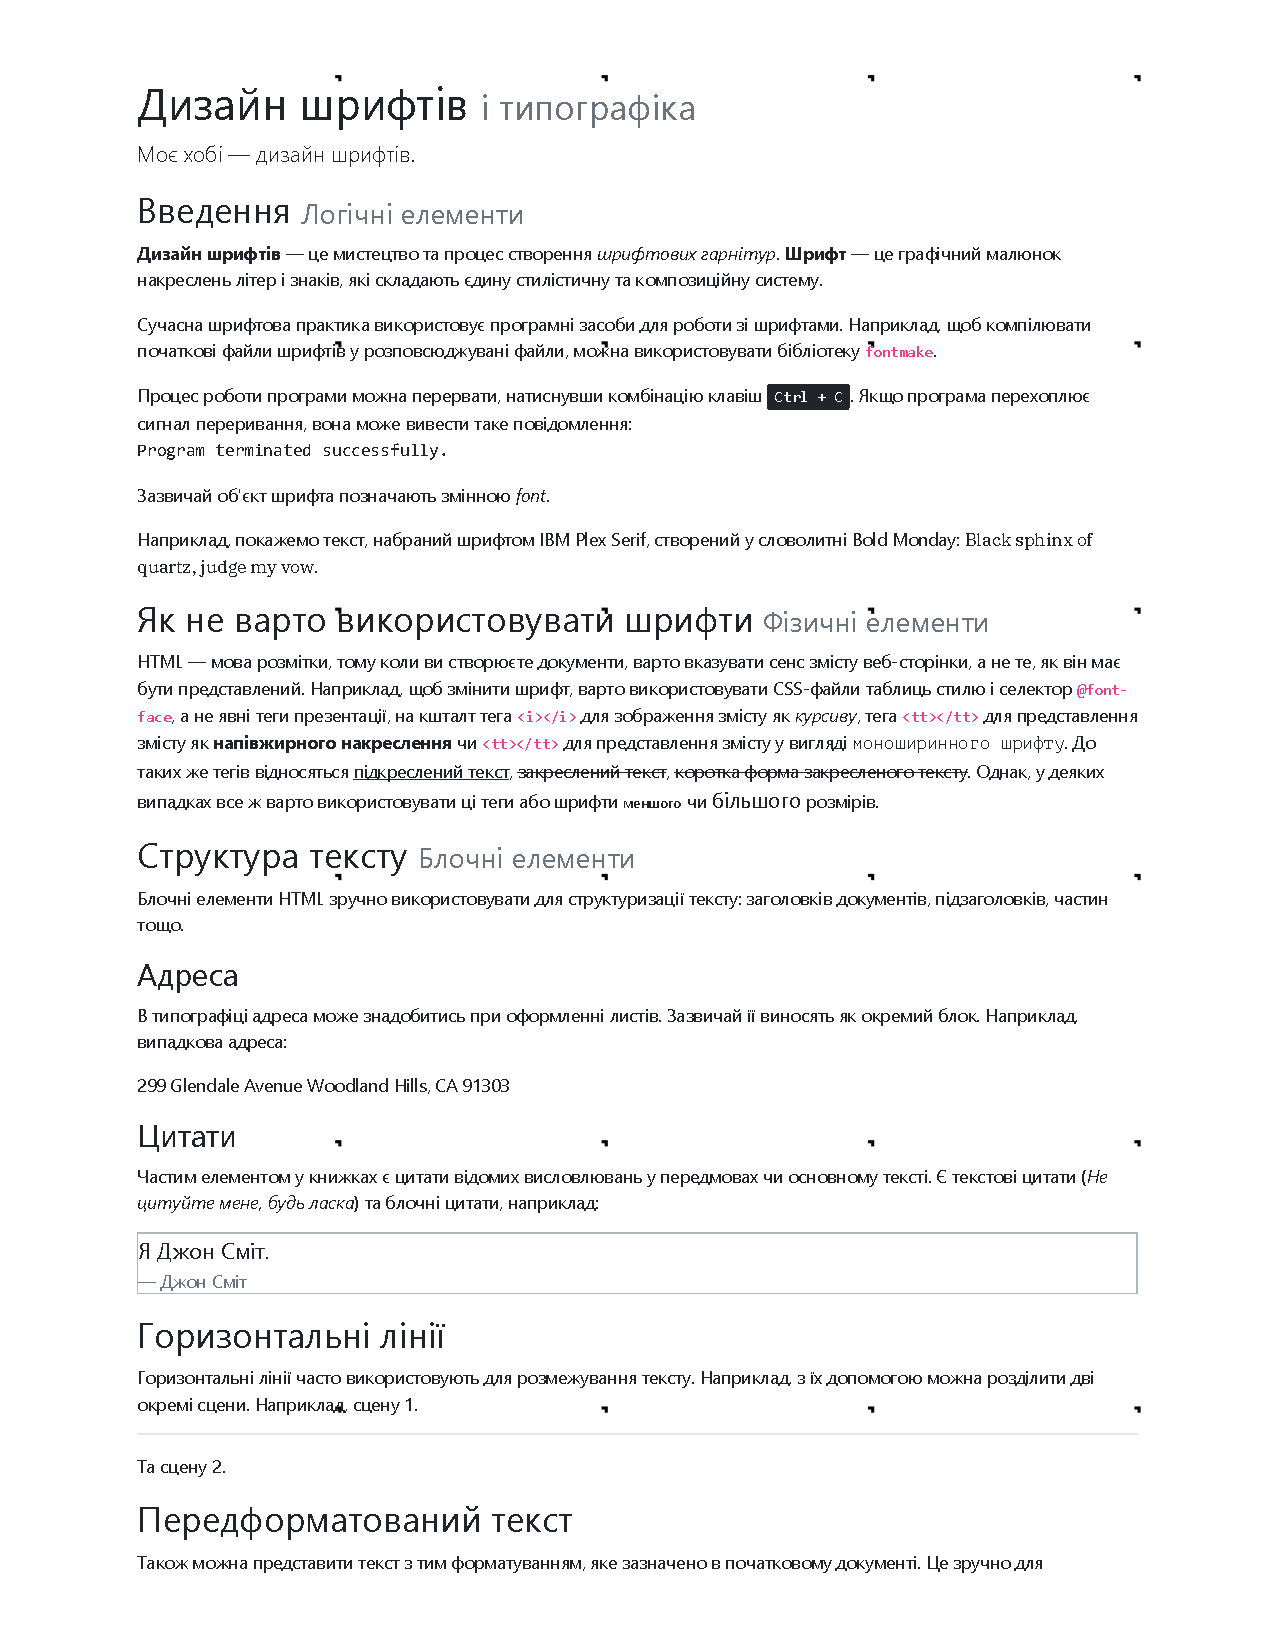
\includepdf[pages=-]{assets/webdoc.pdf}

\end{document}
